\documentclass[dvipdfmx,10pt]{beamer}
%%%% Packages %%%%%
 \usepackage{graphicx}
\usepackage{skak}
% \usepackage{amsmath,amssymb,amsthm}
% \usepackage{multirow}
% \usepackage{url}
% \usepackage{tikz}
% \usepackage{alltt}
% \usepackage{bm}
% \usepackage{listings,jlisting}
% \usepackage{listings}
% \lstset{
%  basicstyle=\ttfamily\scriptsize,
%  keepspaces=true,
%  escapechar=|,
%  columns=[l]{fullflexible}
% }

%%%% Fonts %%%%%
\renewcommand{\kanjifamilydefault}{\gtdefault}
% \usepackage{otf} % otfパッケージ
\usepackage{tikz}
\usetikzlibrary{positioning}
\usepackage[deluxe]{otf} 
\usepackage{txfonts} % 数式・英文ローマン体を Lxfont にする
% \usepackage[T1]{fontenc} % 8bit フォント
% \usepackage{minijs}
% \usepackage{textcomp} % 欧文フォントの追加
% \usepackage[utf8]{inputenc} % 文字コードをUTF-8

%%%% Beamer %%%%%
\usetheme{Madrid}
\useinnertheme{rectangles}
%\useoutertheme{smoothbars}
\setbeamercolor{enumerate}{fg=white, bg=black}
\usefonttheme{professionalfonts}
\setbeamertemplate{frametitle}[default][center]
\setbeamertemplate{navigation symbols}{}
% \setbeamercovered{transparent} % 好みに応じてどうぞ
\setbeamertemplate{footline}[frame number]
\setbeamercolor{page number in head/foot}{fg=black} % ページ数を表示する
% \setbeamerfont{footline}{size=\normalsize,series=\bfseries}
\setbeamerfont{footline}{size=\scriptsize,series=\mdseries}
\setbeamercolor{footline}{fg=black,bg=black}
\setbeamertemplate{blocks}[rounded][shadow=true]
\setbeamertemplate{items}[ball]
% exclude apprendix slides from framenumber %
\newcommand{\backupbegin}{
   \newcounter{framenumberappendix}
   \setcounter{framenumberappendix}{\value{framenumber}}
}
\newcommand{\backupend}{
   \addtocounter{framenumberappendix}{-\value{framenumber}}
   \addtocounter{framenumber}{\value{framenumberappendix}} 
}

% \setbeamertemplate{enumerate items}[default]
% \setbeamerfont{alerted text}{series=\bfseries}
\begin{document}
\title{解集合プログラミングを用いた\\クイーン支配問題の解法に関する考察}
\author{加藤聖人}
\date{2021年度番原研中間発表会\\2021年12月3日}
\institute{番原研究室}

%
%表紙
%

\begin{frame}\frametitle{}
 \titlepage
\end{frame}

%
%支配集合問題について
%

\begin{frame}\frametitle{支配集合問題}
 \begin{block}{支配集合}
  グラフ$G=(V,E)$の頂点の部分集合$S\subset V$とその隣接頂点との和集合が$V$と一致する時,$S$を$V$の\structure{支配集合}という.
  \begin{itemize}
   \item サイズが最小の支配集合をグラフ$G$の\structure{最小支配集合}という.
   \item 最小支配集合のサイズをグラフ$G$の\alert{支配数}と呼び,$\gamma (G)$で表す.
  \end{itemize}
 \end{block}
 \begin{block}{支配集合問題 (入力: グラフ$G$,正の整数$k$)}
  グラフ$G$と正の整数$k$が与えられた時,サイズが$k$の$G$の支配集合が存在するかどうかを判定する問題を\structure{支配集合問題}という.
  \begin{itemize}
   \item 支配集合問題はNP完全であることが知られている.
  \end{itemize}
 \end{block}
\end{frame}

%
%クイーン支配問題
%

\begin{frame}\frametitle{クイーン支配問題}
 \begin{block}{}
  サイズ$n\times n$のクイーングラフ$Q_n$と正の整数$k$が与えられたとき,サイズ$k$の支配集合が存在するかどうかを判定する問題を\structure{クイーン支配問題}と呼ぶ.
  \begin{itemize}
   \item クイーングラフ$Q_n$は$n \times n$のチェス盤において各マスを頂点とし,クイーンが移動できるマス同士が辺で繋がったグラフである.
   \item つまり,$n \times n$の盤面に$k$個のクイーンを置いたとき,クイーンを移動させて全てのマスにアタックできるかを判定する.
  \end{itemize}
 \end{block}
 \begin{block}{}
  クイーングラフの支配数は[Jaenisch,1862]で$\gamma (Q_{8})=5$が示されてから研究されており,$n=3,11$を除いて$n \leq 132$で $\lceil n/2 \rceil \leq \gamma(Q_{n}) \leq \lceil n/2 \rceil +1$であることが証明されている[\"{O}sterg{\aa}rd,Weakley,2001].$1\leq n \leq 20$のクイーングラフの支配数は以下である.
  \begin{table}[hbtp]
   \centering
   \begin{tabular}{|c|c||c|c||c|c||c|c|} \hline
    $n$ & $\gamma(Q_{n})$ & $n$ & $\gamma(Q_{n})$ &$n$ & $\gamma(Q_{n})$ &$n$ & $\gamma(Q_{n})$ \\ \hline
    1 &1 &6 &3 &11 &5 &16 &9 \\ \hline
    2 &1 &7 &4 &12 &6 &17 &9 \\ \hline
    3 &1 &8 &5 &13 &7 &18 &9 \\ \hline
    4 &2 &9 &5 &14 &8 &19 &10 \\ \hline
    5 &3 &10 &5 &15 &9 &20 &11 \\ \hline
   \end{tabular}
  \end{table}
 \end{block}
\end{frame}

%
%クイーングラフの支配集合の例
%

\begin{frame}\frametitle{クイーングラフの支配集合}
 \begin{exampleblock}{例}
  下の図は$Q_8$の最小支配集合の例である.5個のクイーンを置いたとき,クイーンを移動させてすべてのマスにアタック可能である.また,4個以下のクイーンを置いたとき,クイーンを移動させて全てのマスにアタックすることは不可能である.
  \begin{center}
   \scalebox{0.5}{
   \begin{tikzpicture}
 \draw (0,0)--(8,0);
 \draw (0,1)--(8,1);
 \draw (0,2)--(8,2);
 \draw (0,3)--(8,3);
 \draw (0,4)--(8,4);
 \draw (0,5)--(8,5);
 \draw (0,6)--(8,6);
 \draw (0,7)--(8,7);
 \draw (0,8)--(8,8);
 \draw (0,0)--(0,8);
 \draw (1,0)--(1,8);
 \draw (2,0)--(2,8);
 \draw (3,0)--(3,8);
 \draw (4,0)--(4,8);
 \draw (5,0)--(5,8);
 \draw (6,0)--(6,8);
 \draw (7,0)--(7,8);
 \draw (8,0)--(8,8);
 \draw (0,0)--(0,8);
 %\fill[red] (4.5,7.5) circle (0.3);
 \draw[red] (4.5,0.5)--(4.5,7.5);
 \draw[red] (0.5,7.5)--(7.5,7.5);
 \draw[red] (0.5,3.5)--(4.5,7.5);
 \draw[red] (7.5,4.5)--(4.5,7.5);
 %\fill[cyan] (6.5,6.5) circle (0.3);
 \draw[cyan] (0.5,6.5)--(7.5,6.5);
 \draw[cyan] (6.5,0.5)--(6.5,7.5);
 \draw[cyan] (0.5,0.5)--(7.5,7.5);
 \draw[cyan] (5.5,7.5)--(7.5,5.5);
 %\fill[violet] (0.5,3.5) circle (0.3);
 \draw[violet] (0.5,3.5)--(7.5,3.5);
 \draw[violet] (0.5,0.5)--(0.5,7.5);
 \draw[violet] (0.5,3.5)--(4.5,7.5);
 \draw[violet] (0.5,3.5)--(3.5,0.5);
 %\fill[teal] (3.5,2.5) circle (0.3);
 \draw[teal] (0.5,2.5)--(7.5,2.5);
 \draw[teal] (3.5,0.5)--(3.5,7.5);
 \draw[teal] (1.5,0.5)--(7.5,6.5);
 \draw[teal] (0.5,5.5)--(5.5,0.5);
 %\fill[orange] (6.5,0.5) circle (0.3);
 \draw[orange] (0.5,0.5)--(7.5,0.5);
 \draw[orange] (6.5,0.5)--(6.5,7.5);
 \draw[orange] (6.5,0.5)--(0.5,6.5);
 \draw[orange] (6.5,0.5)--(7.5,1.5);
 \fill[red] (4.5,7.5) \symqueen ;
 \fill[cyan] (6.5,6.5) circle (0.35);
 \fill[violet] (0.5,3.5) circle (0.35);
 \fill[teal] (3.5,2.5) circle (0.35);
 \fill[orange] (6.5,0.5) circle (0.35);
\end{tikzpicture}
   }
  \end{center}
 \end{exampleblock}
\end{frame}

%
%ASPについて
%

 \begin{frame}\frametitle{解集合プログラミング(Answer Set Programming; ASP)}
  \begin{block}{ASPとは}
   \begin{itemize}
    \item \structure{ASP言語}は一階論理に基づいた知識表現言語の一種である.
    \item \structure{ASPシステム}は論理プログラムから安定モデル意味論[Gelfond and Lifschitz '88]に基づく解集合を計算するシステムである.
    \item 近年ではSAT技術を応用した高速ASPシステムが実現され,システム検証,プランニング,システム生物学など様々な分野への応用が拡大している.
   \end{itemize}
  \end{block}
  \begin{alertblock}{クイーン支配問題に対してASPを用いる利点}
   \begin{itemize}
    \item ASPの高い表現力により,クイーン支配問題の制約を簡潔に記述可能.
    \item 探索ヒューリスティックスを容易に変更できる.
   \end{itemize}
  \end{alertblock}
 \end{frame}
 
 %
 %研究目的
%

\begin{frame}\frametitle{研究目的}
 \begin{alertblock}{研究目的}
  ASPを用いて,クイーン支配問題を高速に解く符号化を提案する.
 \end{alertblock}
 \begin{block}{研究内容}
  \begin{itemize}
   \item 3種類の符号化の提案.
	 \begin{itemize}
	  \item \structure{基本制約モデル}:マス$(i,j)$のクイーンの有無を表す変数のみを用いてクイーンの移動と個数の制約を表現.\vspace{2mm}
	  \item \structure{改良制約モデル1}:基本モデルに加えて,行,列,対角線ごとのクイーンの存在の有無を表す補助ブール変数を導入し,重複する変数をまとめる.\vspace{2mm}
	  \item \structure{改良制約モデル2}:改良制約モデル1を拡張し,行,列,対角線ごとのクイーンの個数を表す補助ブール変数を用いてクイーンの総数に関する制約を追加.\vspace{2mm}
	 \end{itemize}
   \item 各種符号化の評価実験.
  \end{itemize}
 \end{block}
\end{frame}

%
%符号化1/2
%

\begin{frame}\frametitle{符号化(1/2)}
 \begin{block}{基本制約モデル}
  \begin{itemize}
   \item サイズ$n$のクイーングラフ$Q_{n}$上の各マスを$(i,j)$と表す.
   \item マス$(i,j)$のクイーンの有無をブール変数$q_{ij}$で表す.
   \item クイーングラフ上のクイーンの総数が$k$個である制約を加える.
   \item 各マス$(i,j)$について,\structure{自身とその隣接頂点にクイーンがひとつ以上存在する}制約を加える.
  \end{itemize}
 \end{block}
 \begin{block}{改良制約モデル1}
  \begin{itemize}
   \item サイズ$n$のクイーングラフ$Q_{n}$上の各マスを$(i,j)$と表す.
   \item マス$(i,j)$のクイーンの有無をブール変数$q_{ij}$で表す.
   \item クイーングラフ上のクイーンの総数が$k$個である制約を加える.
   \item マス$(i,j)$に対して,\structure{各列,各行,各対角線上のクイーンの有無}を補助ブール変数$r_{i},c_{j},u_{i+j},d_{i-j}$で表す.
   \item 各マス$(i,j)$について,その\structure{行,列,対角線上にクイーンがひとつ以上存在する}制約を追加する.
  \end{itemize}
 \end{block}
\end{frame}

%
%符号化2/2
%

\begin{frame}\frametitle{符号化(2/2)}
 \begin{block}{改良制約モデル2}
  \begin{itemize}
   \item サイズ$n$のクイーングラフ$Q_{n}$上の各マスを$(i,j)$と表す.
   \item マス$(i,j)$のクイーンの有無をブール変数$q_{ij}$で表す.
   \item マス$(i,j)$に対して,各列,各行,各対角線上にそれぞれちょうど$a$個のクイーンが配置されているかどうかを補助ブール変数$r(i,a),c(j,a),u(i+j,a),d(i-j,a)$で表す.
   \item \alert{行方向,列方向,対角線方向それぞれに対して,クイーンの総数が$k$個}である制約を追加する.
  \end{itemize}
 \end{block}
\end{frame}

%
%改良制約モデル2の追加制約
%

\begin{frame}\frametitle{改良制約モデル2における行方向の追加制約による推論}
 \begin{block}{}
  \begin{description}
   \item[(追加制約1)] $r_{i}=\sum\limits_{(i',j')\in \mbox{行}i} q_{i'j'} \;\;\;\;\; (1 \leq i \leq n)$:行$i$のクイーンの個数を$r_i$とする.
   \item[(追加制約2)] $\sum\limits_{i=1}^{n}r_{i} = k$:行ごとのクイーンの合計は盤面全体の数に一致する.
  \end{description}
 \end{block}
 \begin{exampleblock}{例:$n=5,k=3$のとき}
  \begin{columns}
   \begin{column}{0.30\textwidth}
    \centering
    %%%%%%%%%%%%%%%%%%%%%%%%%%%%%%%%%%%%%%%%%%%%%%%%%%
% 実行例(t=0) (第6章で使う)
%%%%%%%%%%%%%%%%%%%%%%%%%%%%%%%%%%%%%%%%%%%%%%%%%%

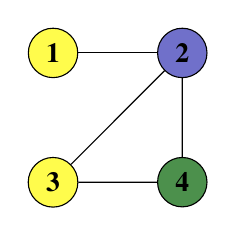
\begin{tikzpicture}[scale=0.6]

  % 設定
  \tikzset{node/.style={circle,draw=black}}
 
  \definecolor{col_r}{RGB}{230,0,18}
  %\definecolor{col_b}{RGB}{0,104,183}
  \definecolor{col_b}{RGB}{51,51,179}
  \definecolor{col_y}{RGB}{255,251,0}
  \definecolor{col_g}{RGB}{0,96,0}
 
  % 補助線
  % \draw [help lines,blue] (0,0) grid (20,6);
 
  % node %
  \node[node, fill=col_y!70] (node1){\textbf{1}};
  \node[node, fill=col_b!70, right=of node1] (node2){\textbf{2}};
  \node[node, fill=col_y!70, below=of node1] (node3){\textbf{3}};
  \node[node, fill=col_g!70, below=of node2] (node4){\textbf{4}};
 
  \foreach \u / \v in {node1/node2, node2/node3, node2/node4, node3/node4}
  \draw (\u) -- (\v);
 \end{tikzpicture}
 
 %%%%%%%%%%%%%%%%%%%%%%%%%%%%%%%%%%%%%%%%%%%%%%%%%%%%%%%%%%
 %%% Local Variables:
 %%% mode: japanese-latex
 %%% TeX-master: paper.tex
 %%% End:
 
   \end{column}
   \begin{column}{0.30\textwidth}
    \centering
    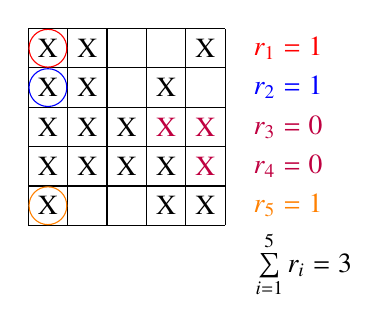
\begin{tikzpicture}
 \draw (0,0)--(2.5,0);
 \draw (0,0.5)--(2.5,0.5);
 \draw (0,1.0)--(2.5,1.0);
 \draw (0,1.5)--(2.5,1.5);
 \draw (0,2.0)--(2.5,2.0);
 \draw (0,2.5)--(2.5,2.5);
 \draw (0,0)--(0,2.5);
 \draw (0.5,0)--(0.5,2.5);
 \draw (1.0,0)--(1.0,2.5);
 \draw (1.5,0)--(1.5,2.5);
 \draw (2.0,0)--(2.0,2.5);
 \draw (2.5,0)--(2.5,2.5);
 \node (X) at (0.25,0.25) {X};
 \draw [orange] (0.25,0.25) circle[radius = 0.24];
 \node (X) at (0.25,0.75) {X};
 \node (X) at (0.25,1.25) {X};
 \node (X) at (0.25,1.75) {X};
 \draw [blue] (0.25,1.75) circle[radius = 0.24];
 \node (X) at (0.25,2.25) {X};
 \draw [red] (0.25,2.25) circle[radius = 0.24];
 \node (X) at (0.75,2.25) {X};
 \node (X) at (0.75,0.75) {X};
 \node (X) at (0.75,1.25) {X};
 \node (X) at (0.75,1.75) {X};
 \node (X) at (1.25,0.75) {X};
 \node (X) at (1.25,1.25) {X};
 \node (X) at (1.75,0.25) {X};
 \node (X) at (1.75,0.75) {X};
 \node (X) at (1.75,1.25) {\color{purple}X};
 \node (X) at (1.75,1.75) {X};
 \node (X) at (2.25,0.25) {X};
 \node (X) at (2.25,0.75) {\color{purple}X};
 \node (X) at (2.25,1.25) {\color{purple}X};
 \node (X) at (2.25,2.25) {X};
 \node (A) at (3.30,2.25) {\color{red}$r_{1} = 1$};
 \node (B) at (3.30,1.75) {\color{blue}$r_{2} = 1$};
 \node (M) at (3.30,1.25) {\color{purple}$r_{3} = 0$};
 \node (M) at (3.30,0.75) {\color{purple}$r_{4} = 0$};
 \node (C) at (3.30,0.25) {\color{orange}$r_{5} = 1$};
 \node (D) at (3.50,-0.50) {$\sum\limits_{i=1}^{5}r_{i}=3$};
\end{tikzpicture}
   \end{column}
  \end{columns}
  \begin{itemize}
   \item 左の図の状態から,追加制約2によって右の状態を推論できる.
  \end{itemize}
 \end{exampleblock}
\end{frame}

%
%実験内容
%
 
\begin{frame}\frametitle{実験内容}
 \begin{block}{}
  ASPソルバーにおいて提案した各制約モデルを用い,正の整数$(n,k)$を入力としてサイズ$k$の$Q_{n}$の支配集合の有無を判定した.
  \begin{itemize}
   \item $10 \leq n \leq 20$
   \item $k=\gamma(Q_{n})$:SATと$k=\gamma(Q_{n})-1$:UNSATの2種類の計22問を判定する.
   \item 使用ASPソルバ: \textit{clingo-5.5.0}
	 \begin{itemize}
	  \item \textit{configuration}は\textit{trendy, handy}を使用.
	 \end{itemize}
   \item 実行環境: Mac mini, 3.2GHz 6コア Intel Core i7, 64GBメモリ
   \item 制限CPU時間: 3600 (sec)
  \end{itemize}
 \end{block}
\end{frame}

%
%実験結果
%

\begin{frame}\frametitle{実験結果}
 \begin{itemize}
  \item 各制約モデルに対して時間内の判定ができた数を比較する.
 \end{itemize}
 \begin{block}{}
  \begin{table}[ht]
   \centering
   \begin{tabular}{c|c|c}
    &SAT &UNSAT \\ \hline
    基本制約モデル &3 &3 \\
    改良制約モデル1 &5 &3 \\
    改良制約モデル2 &{\color{red}7} &{\color{red}3} \\ \hline
   \end{tabular}
  \end{table}
  \begin{itemize}
   \item $k=\gamma (Q_{n})$の問題では,\structure{改良制約モデル2}が$n=16$まで解を発見するなど良い性能を示した.
   \item $k=\gamma (Q_{n})-1$の問題ではどのモデルでも解けた問題数は変わらなかったが,UNSATを導くまでにかかった時間では\structure{改良制約モデル2}が良い性能を示した.
  \end{itemize}
 \end{block}
\end{frame}

\begin{frame}\frametitle{実験結果}
 \begin{block}{$k=\gamma(Q_{n})$}
  \begin{table}[ht]
   \centering
   \begin{tabular}{c|c|r|r|r}
   n &k &基本制約モデル &改良制約モデル1 &改良制約モデル2 \\ \hline
   10 & 5 & 8.467 & 21.232 & 3.005 \\
   11 & 5 & 189.473 & 123.488 & 32.540 \\
   12 & 6 & 1349.260 & 56.468 & 2.147 \\
   13 & 7 & T.O. & 1281.823 & 22.412 \\
   14 & 8 & T.O. & 772.276 & 10.044 \\
   15 & 9 & T.O. & T.O. & 275.683 \\
   16 & 9 & T.O. & T.O. & 734.878 \\
   17 & 9 & T.O. & T.O. & T.O. \\
   \end{tabular}
  \end{table}
 \end{block}
 \begin{block}{$k=\gamma(Q_{n})-1$}
  \begin{table}[ht]
   \centering
   \begin{tabular}{c|c|r|r|r}
    n & k & 基本制約モデル & 改良制約モデル1 & 改良制約モデル2 \\ \hline
    10 & 4 & 6.520 & 1.538 & 1.538 \\
    11 & 4 & 16.468 & 2.894 & 1.694 \\
    12 & 5 & 3071.506 & 2718.137 & 187.554 \\
    13 & 6 & T.O. & T.O. & T.O. \\  
   \end{tabular}
  \end{table}
 \end{block}
\end{frame}

\begin{frame}\frametitle{まとめと今後の課題}
 \begin{block}{まとめ}
  \begin{itemize}
   \item クイーン支配問題に対して,3種類の符号化を実装した,
   \item 各行,各列,各対角線ごとのクイーンの総数に関する制約を追加することにより,ASPソルバでの高速化を実現した.
  \end{itemize}
 \end{block}
 \begin{alertblock}{今後の課題}
  \begin{itemize}
   \item クイーン支配問題をより効率的に解くASP符号化の考案.
   \item 新たに考案した各種符号化の評価実験.
  \end{itemize}
 \end{alertblock}
\end{frame}

%%%% 補助スライド

\begin{frame}{~}
 \centering
 - 補足用 -
\end{frame} 

\begin{frame}{補足 : スマートグリッド}
 \begin{itemize}
  \item \structure{スマートグリッド}とは,電力の供給側,需要側において双方向の
		やり取りを可能にする次世代の\structure{賢い}電力網である.
  \item 従来と違い,通信技術の発達により,使用状況などを
		リアルタイムに把握することが可能となった.
  \item その時に応じた最適な配電網を構成し,制御するといったことが考えられている.
		\begin{itemize}
		 \item 電力需要の変化による,配電ロスの少ない構成.
		 \item 自然エネルギーによる発電量の変動を補う構成.
		\end{itemize}
  \item ASP言語の表現力や拡張性が,こうした条件の追加に活用できる可能性がある.
 \end{itemize}
\end{frame}

%%%%%%%%%%%%%%%%%%%%%%%%%%%%%%%%%%%%%%%%%%%%%%%%%%
%% 電気制約
%%%%%%%%%%%%%%%%%%%%%%%%%%%%%%%%%%%%%%%%%%%%%%%%%%
\begin{frame}{補足 : 電気制約}
 \begin{itemize}
  \item \alert{電気制約}は,送電する電流$\cdot$電圧の適正範囲を保証する制約.
  \begin{itemize}
   \item 供給経路の各区間で許容電流を超えない.
   \item 電気抵抗による電圧降下が許容範囲を超えない.
   \item etc.
  \end{itemize}
  \item 電流と電圧が影響し合う\structure{実数ドメイン上の制約}によって表される.
		% \begin{itemize}
		%  		 \item 送電システム上の条件など.
		% \end{itemize}
  \item 実数ドメイン上の制約は,純粋なASPのみで扱うのは\alert{困難}.
		\begin{itemize}
		 \item 緩和問題として,変電所から供給できる家庭の数に上限をつける.
		 \item ASPMT技術により,ASPで得られた解について,
			   背景理論ソルバーと連携して実数ドメイン上の制約を調べる.
		\end{itemize}
 \end{itemize}
\end{frame}


%%%%%%%%%%%%%%%%%%%%%%%%%%%%%%%%%%%%%%%%%%%%%%%%%%
%% 基礎化
%%%%%%%%%%%%%%%%%%%%%%%%%%%%%%%%%%%%%%%%%%%%%%%%%%
\begin{frame}{補足 : ASPシステム}
 
 \vspace{-0.5cm}

 \begin{figure}[htbp]
  \centering
  %%%%%%%%%%%%%%%%%%%%%%%%%%%%%%%%%%%%%%%%%%%%%%%%%%
%% 基礎化の流れの図
%%%%%%%%%%%%%%%%%%%%%%%%%%%%%%%%%%%%%%%%%%%%%%%%%%
\begin{tikzpicture}

 \definecolor{edge}{RGB}{38,38,134}
 \definecolor{node}{RGB}{220,220,249}

 \definecolor{alert_edge}{RGB}{191,0,0}
 \definecolor{alert_node}{RGB}{249,200,200}

 \definecolor{ex_edge}{RGB}{0,96,0}
 \definecolor{ex_node}{RGB}{230,239,230}

 \def\nodespace{2.4cm}

 \tikzset{block/.style={rectangle, thick, draw=edge, fill=node, text width=3cm, 
 text centered, rounded corners, text width=2cm, minimum height=1.5cm}};

 \tikzset{alertblock/.style={rectangle, thick, draw=alert_edge, fill=alert_node, 
 text width=3cm, text centered, rounded corners, text width=1.5cm, minimum height=1.2cm}};

 \node[block](ikkai){一階ASP\\プログラム};

 \node[rectangle,rounded corners, thick, draw=ex_edge, fill=ex_node, 
 right=0.22*\nodespace of ikkai, minimum width=6cm, minimum height=3cm, 
 text centered, label=ASPシステム](sys){};

 \node[block, right=\nodespace of ikkai](meidai){命題ASP\\プログラム};
 \node[block, right=\nodespace of meidai](ASP){解集合};

 \node[right=0.6*\nodespace of ikkai, text width=1.5cm, 
 text centered, text=red, anchor=south](){基礎化\\ソルバー};
 \node[right=0.4*\nodespace of meidai, text width=1.5cm, 
 text centered, text=red, anchor=south](){解集合\\ソルバー};

 
 \foreach \u / \v / \n in {ikkai/meidai,meidai/ASP}
 \draw [thick,->] (\u) to (\v);

\end{tikzpicture}
 \end{figure}

 \vspace{-0.5cm}

 \begin{exampleblock}{}
  \begin{enumerate}
   \item 一階ASPプログラムを基礎化ソルバーによって,
		 命題ASPプログラムに\alert{基礎化}する.
   \item 命題ASPプログラムについて,SAT技術を応用した解集合ソルバーが解集合を探索する.
  \end{enumerate}
 \end{exampleblock}

\end{frame}


%%%%%%%%%%%%%%%%%%%%%%%%%%%%%%%%%%%%%%%%%%%%%%%%%%
%% ASPのコード
%%%%%%%%%%%%%%%%%%%%%%%%%%%%%%%%%%%%%%%%%%%%%%%%%%
\begin{frame}[fragile]{補足 : 基本符号化のASPプログラム}
 \begin{exampleblock}{}
  \begin{center}
   %%%%%%%%%%%%%%%%%%%%%%%%%%%%%%%%%
   \lstinputlisting[numbers=left,%
   basicstyle=\ttfamily\tiny]{code/srf1.lp}
   %%%%%%%%%%%%%%%%%%%%%%%%%%%%%%%%% 
  \end{center}
 \end{exampleblock}
\end{frame}

\begin{frame}[fragile]{補足 : 改良符号化のASPプログラム}

 \begin{exampleblock}{}
  \begin{center}
   %%%%%%%%%%%%%%%%%%%%%%%%%%%%%%%%%
   \lstinputlisting[numbers=left,%
   basicstyle=\ttfamily\tiny]{code/srf2.lp}
   %%%%%%%%%%%%%%%%%%%%%%%%%%%%%%%%% 
  \end{center}
 \end{exampleblock}

\end{frame}



\end{document}